\documentclass{article}

\usepackage{booktabs}
\usepackage{tabularx}
\usepackage{graphicx}
\usepackage{float}
\usepackage[margin=1in]{geometry}

\input{../../Comments.text}
\input{../../Common.text}

\title{Wireframe Report (CD-Fall)\\\progname}
\author{\authname}
\date{}

\begin{document}

\maketitle

\begin{table}[hp]
\caption{Revision History} \label{TblRevisionHistory}
\begin{tabularx}{\textwidth}{llX}
\toprule
\textbf{Date} & \textbf{Developer(s)} & \textbf{Change}\\
\midrule
Nov 16, 26 & Vedant Patel & Initial version: prototype screenshots\\
... & ... & ...\\
\bottomrule
\end{tabularx}
\end{table}

\newpage

\section{Mock-up}

The screenshots below are from the clickable prototype in
\texttt{docs/CDs/Wireframe/prototype/index.html}. \href{https://raw.githack.com/RishabShine/IDE3.0/main/docs/CDs/Wireframe/prototype/index.html}{\textbf{Click
here to open the prototype in a browser}} (no download needed), or download
the file and double-click it.

\begin{figure}[H]
  \centering
  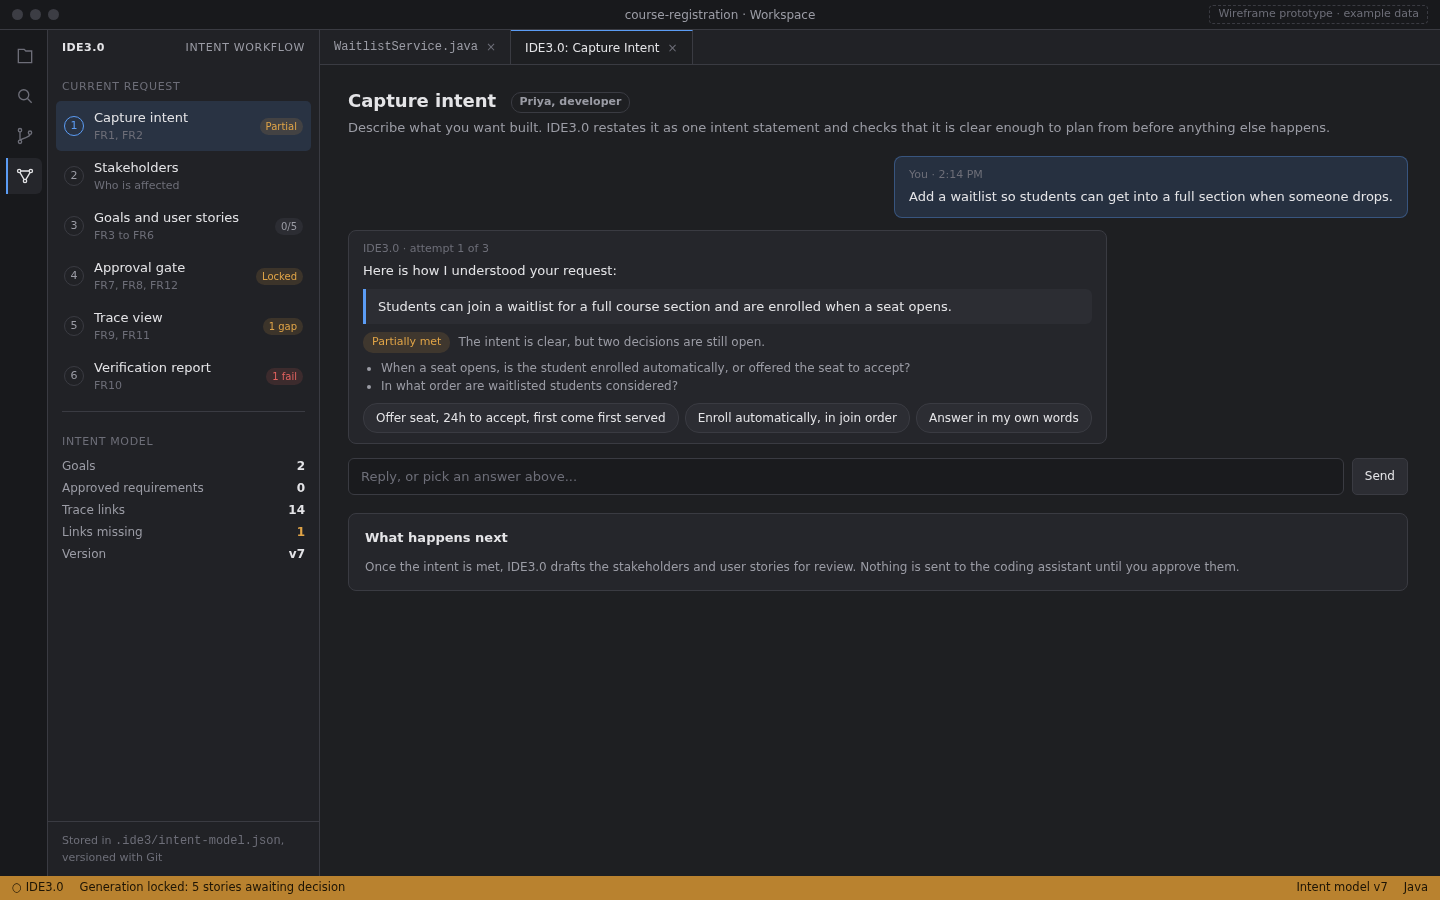
\includegraphics[width=\textwidth]{figures/intent-partial.png}
  \caption{Capture Intent: first attempt, judged partially met.}
\end{figure}

\begin{figure}[H]
  \centering
  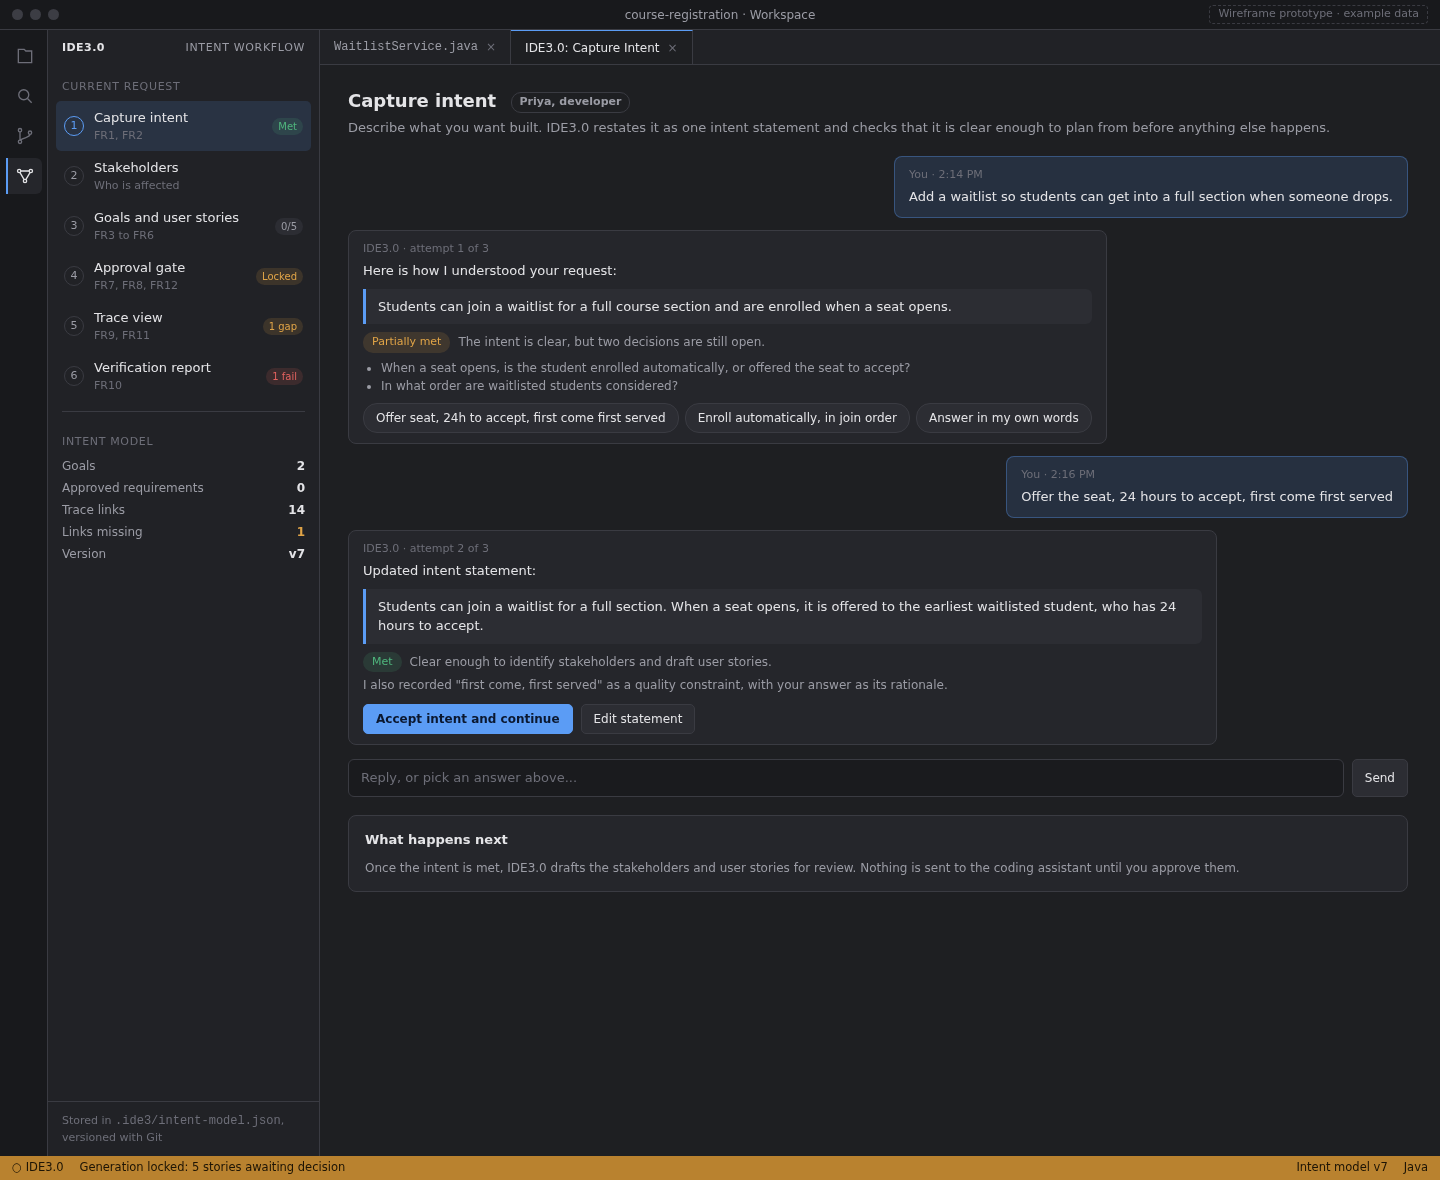
\includegraphics[width=\textwidth]{figures/intent-met.png}
  \caption{Capture Intent: after clarification, judged met.}
\end{figure}

\begin{figure}[H]
  \centering
  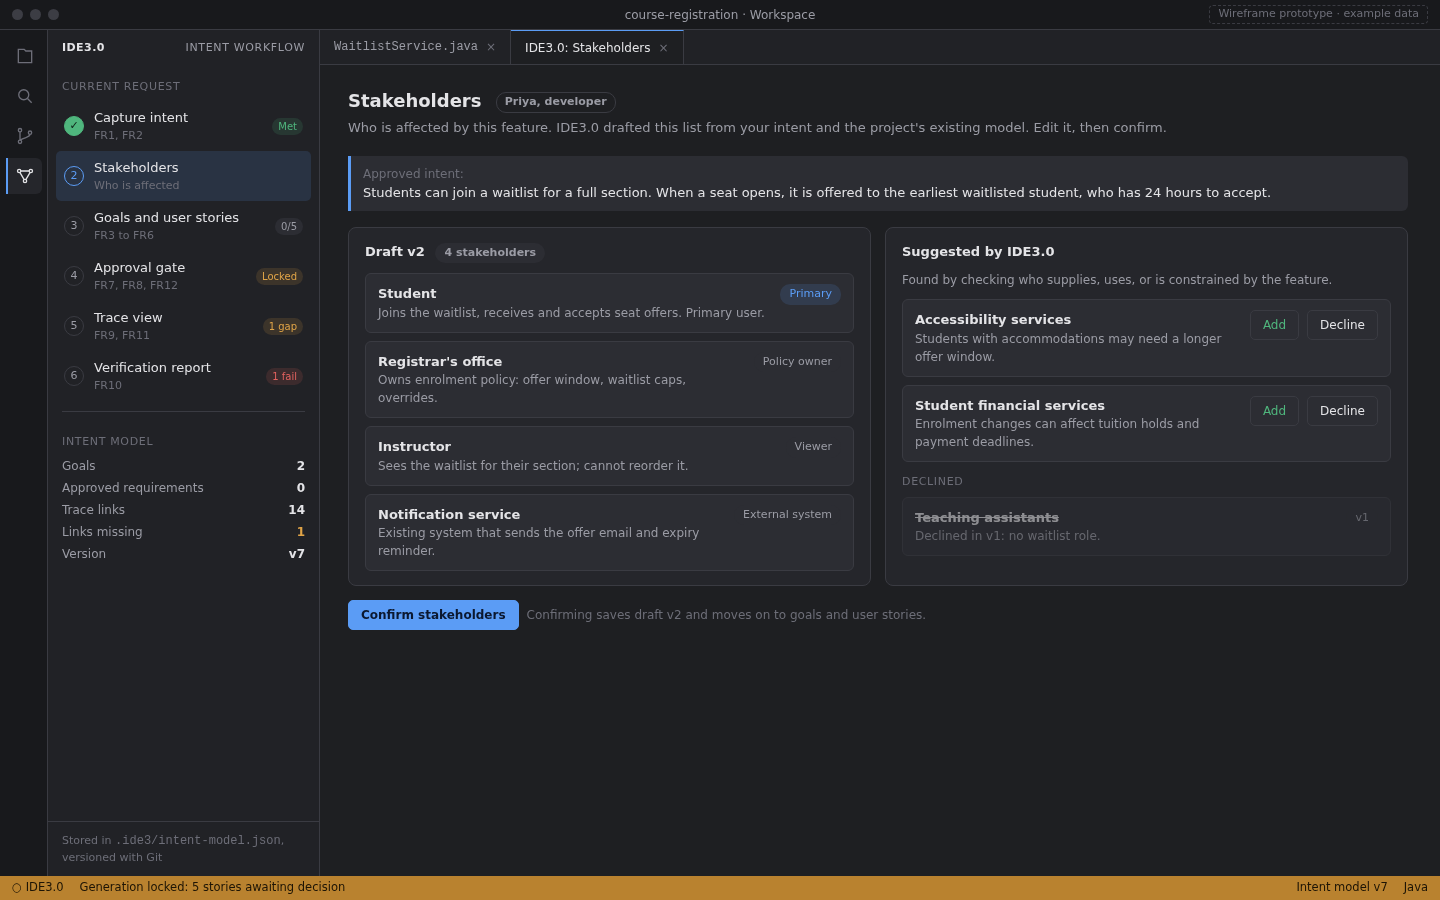
\includegraphics[width=\textwidth]{figures/stakeholders.png}
  \caption{Stakeholders.}
\end{figure}

\begin{figure}[H]
  \centering
  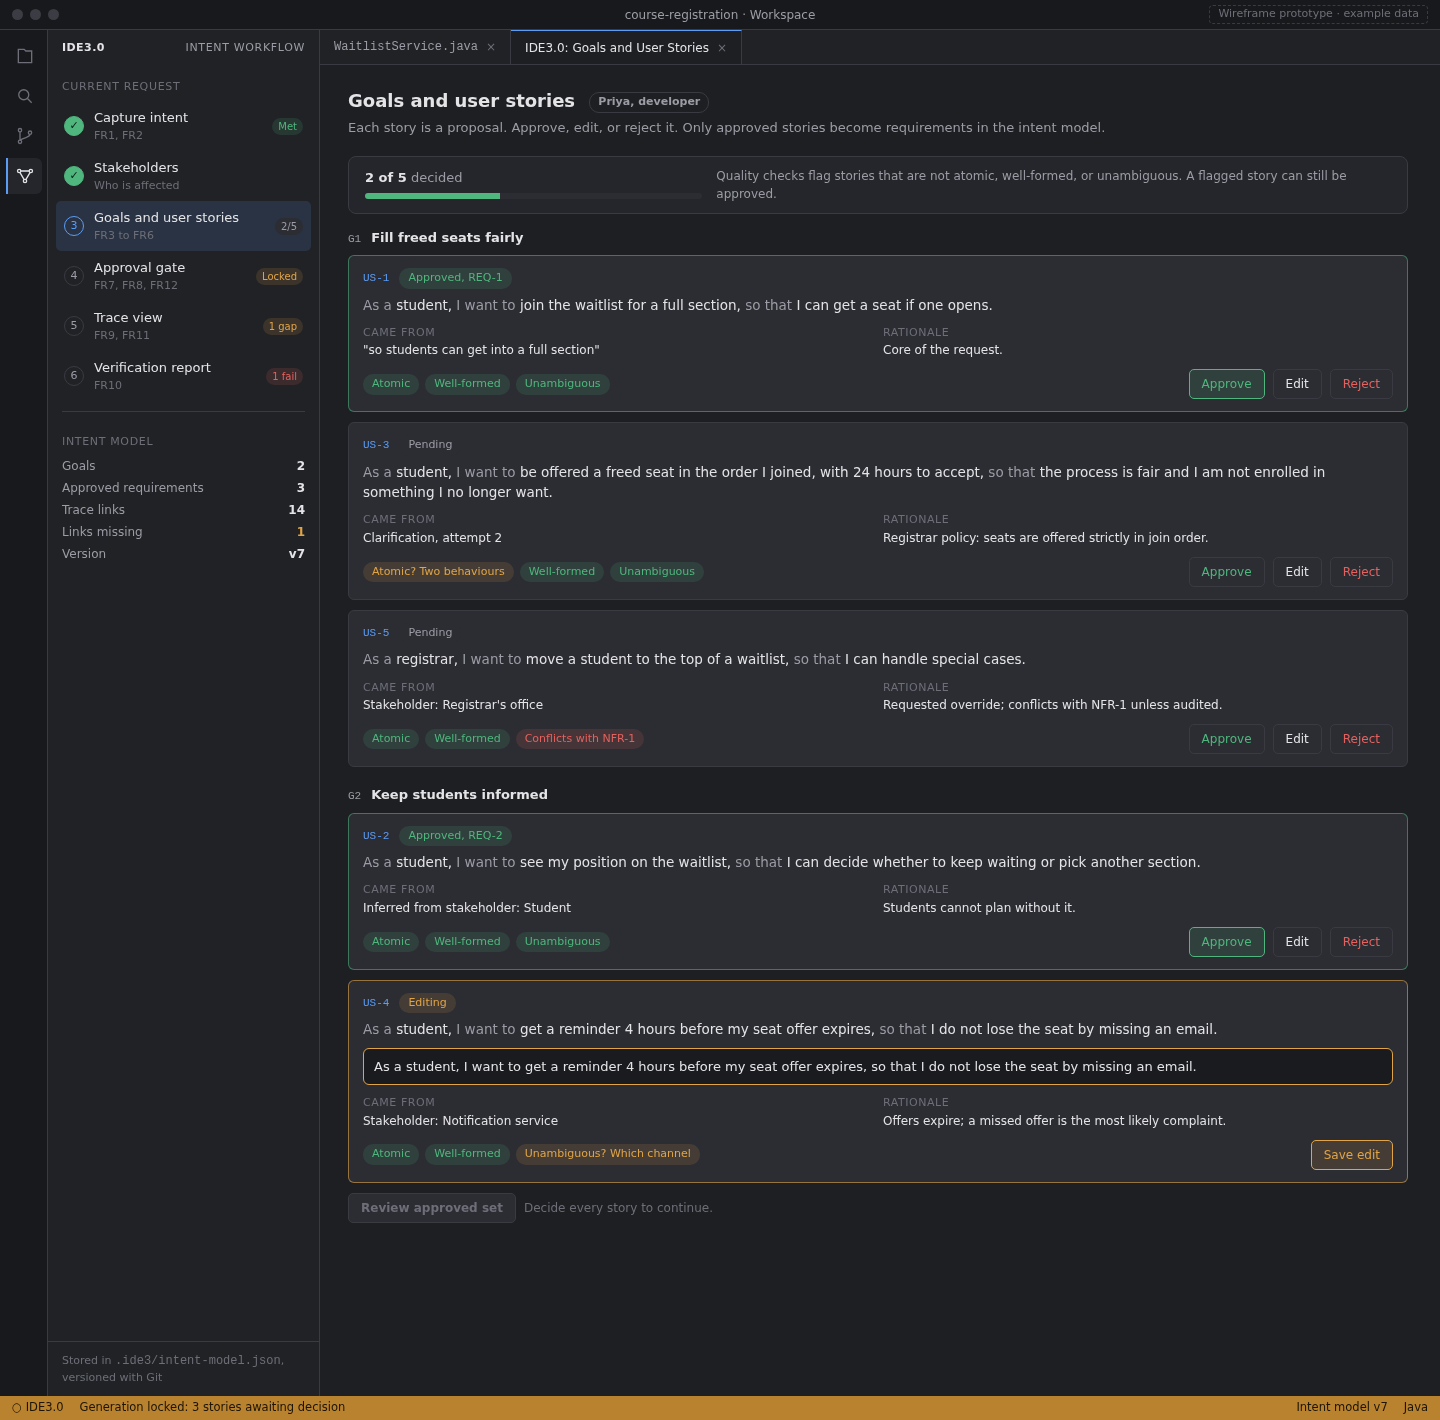
\includegraphics[width=\textwidth]{figures/stories.png}
  \caption{Goals and User Stories.}
\end{figure}

\begin{figure}[H]
  \centering
  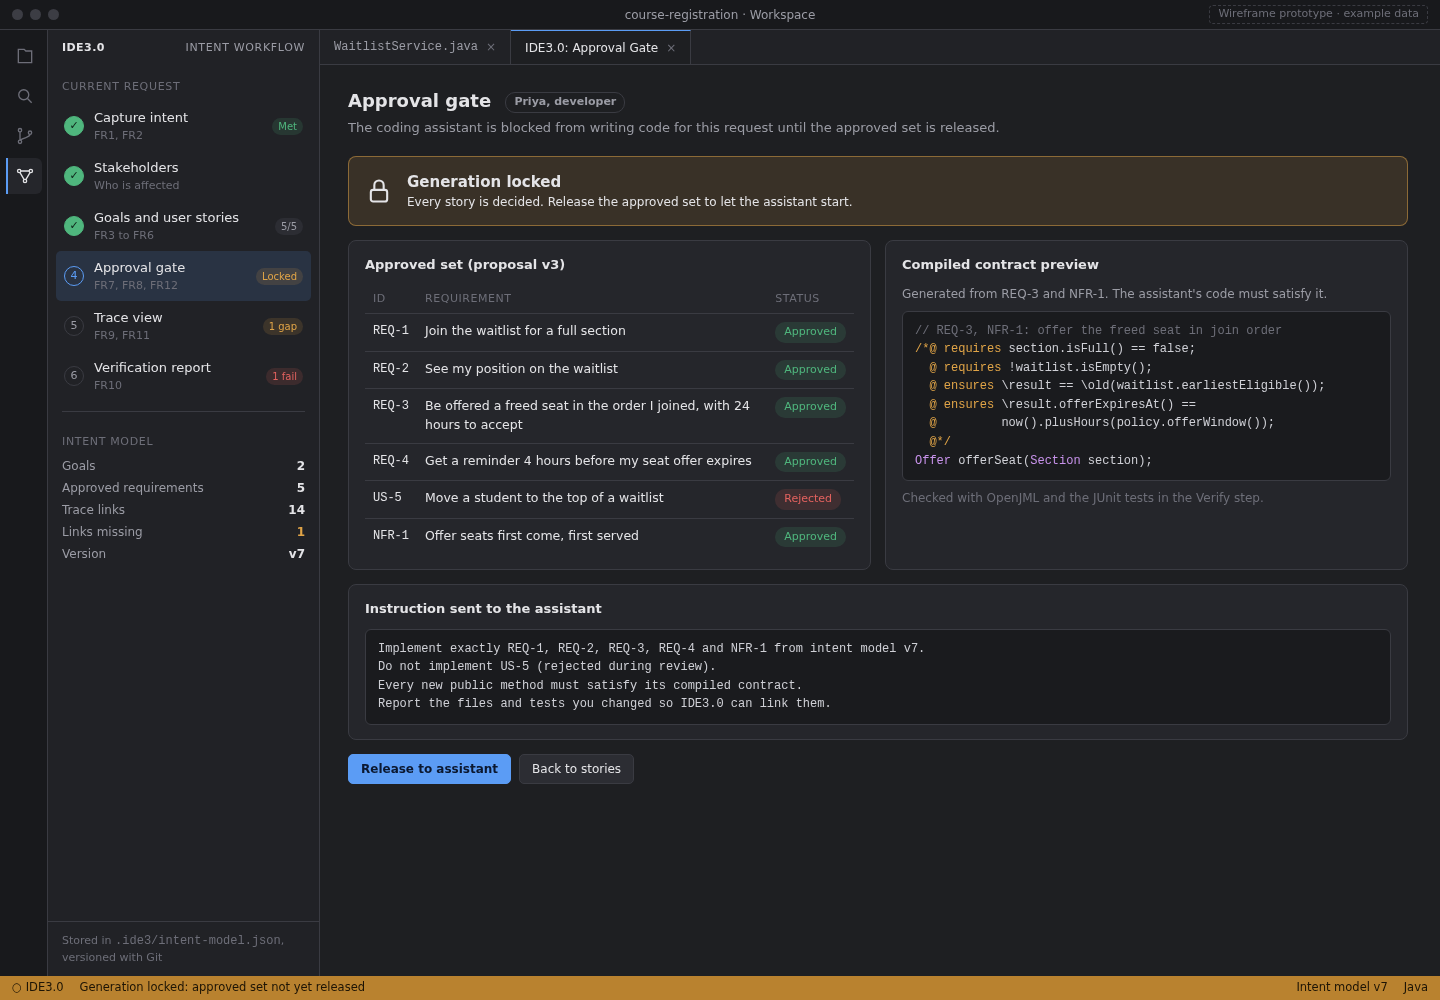
\includegraphics[width=\textwidth]{figures/gate.png}
  \caption{Approval Gate.}
\end{figure}

\begin{figure}[H]
  \centering
  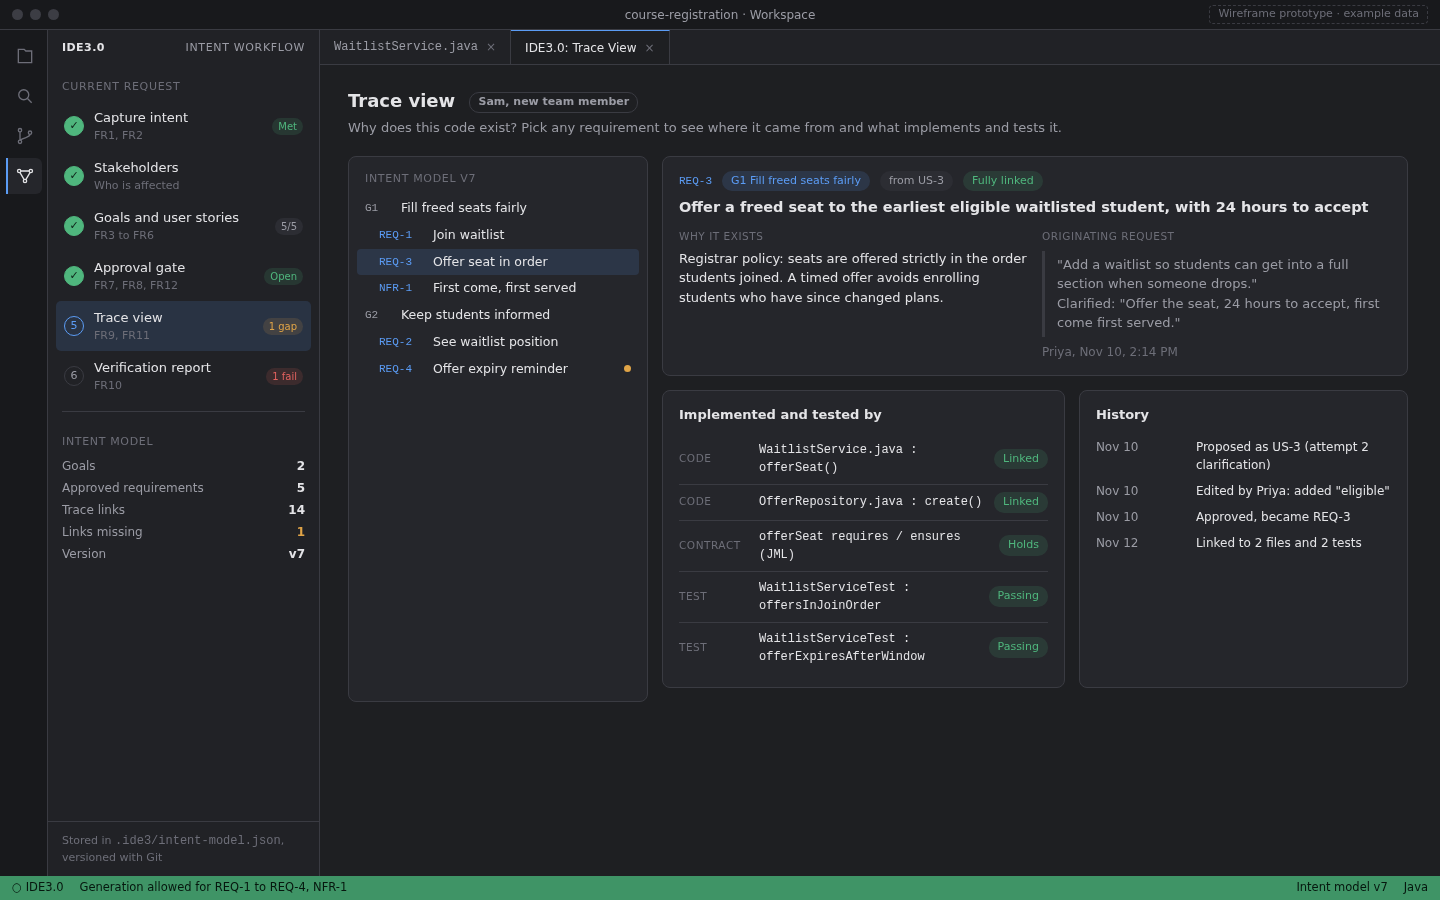
\includegraphics[width=\textwidth]{figures/trace.png}
  \caption{Trace View.}
\end{figure}

\begin{figure}[H]
  \centering
  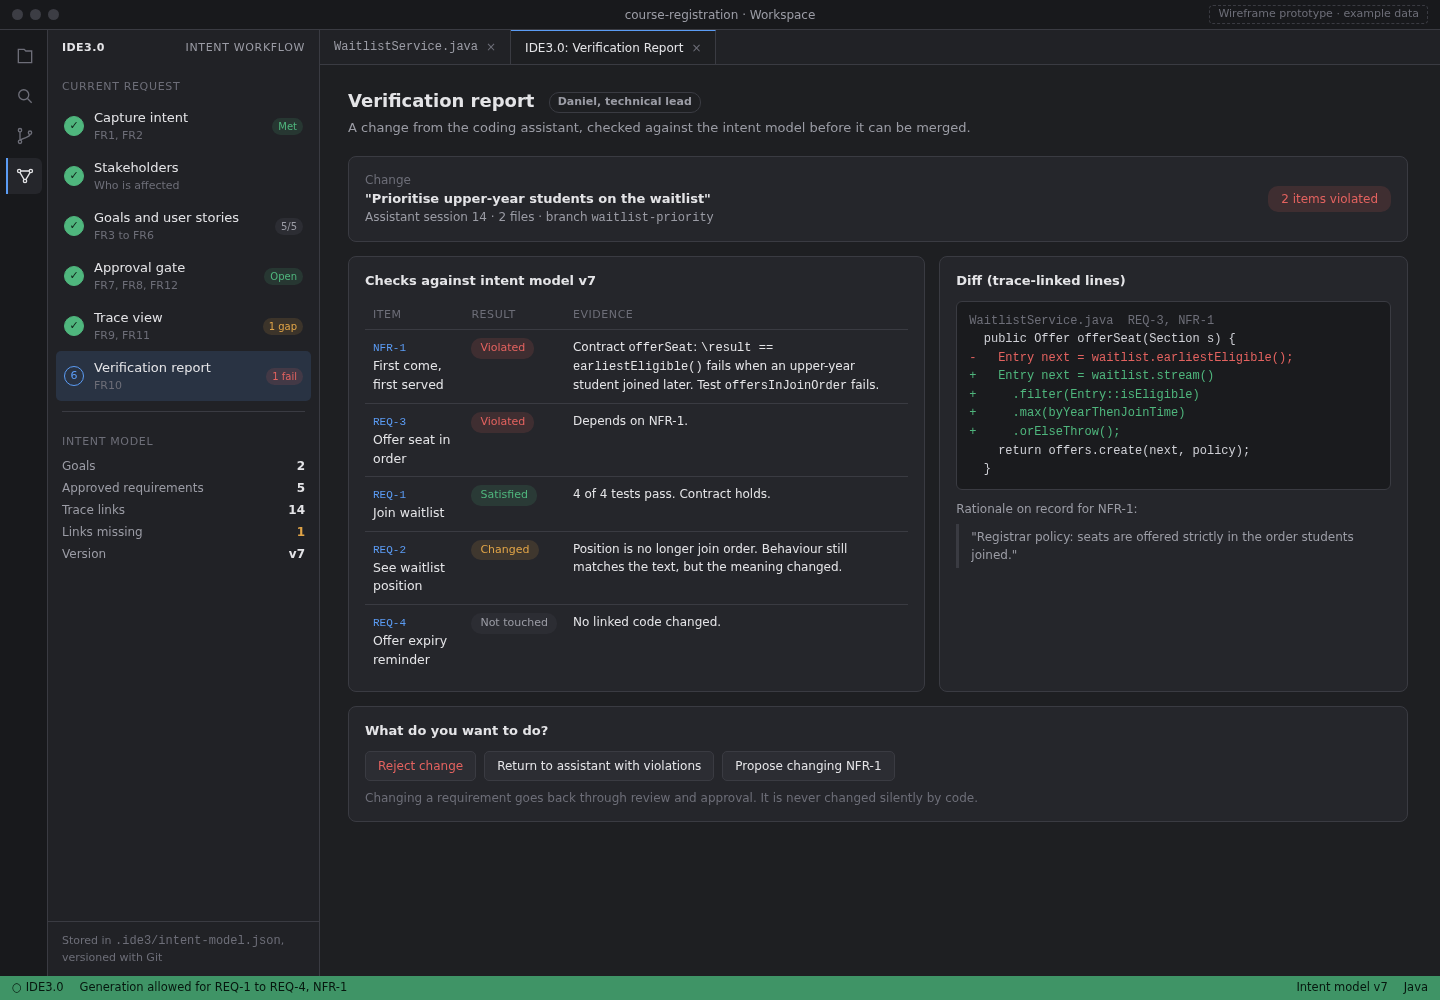
\includegraphics[width=\textwidth]{figures/verify.png}
  \caption{Verification Report.}
\end{figure}

\section{Discussion}

The prototype was shown to classmates in SFWRENG 4G06 on November 16, 2026.
They clicked through the screens and gave informal feedback. Two main
insights came out of the session.

\paragraph{The screens are text heavy.} Classmates felt that several screens
ask the developer to read a lot before they can act. This matters because the
SRS requires a workflow that is simple and easy to learn (EUR1, LR1), and a
developer will skip the review steps if they take too long to read.
\emph{Response:} as the product is built, the team will cut explanatory text
on each screen, lead with the decision the developer has to make, and move
supporting detail (such as rationale and quality checks) behind expandable
sections. This affects the Review Panel module.

\paragraph{There is no introduction to how to use the tool or why.}
Classmates were not sure where to start or what problem the tool solves,
because the prototype opens directly on the first step of the workflow. This
relates to the SRS requirement that a new user can understand the tool with
minimal instruction (LR2). \emph{Response:} the team will add a short
first-run walkthrough that explains the problem \progname{} addresses (losing
the reasons behind AI-generated code) and steps through one example request.
This affects the Host IDE Interface and Review Panel modules.

Both changes will be made as the product is built, and their effect will be
measured in the winter Usability Report (CD-Winter).

\end{document}
